\documentclass[main.tex]{subfiles}

\begin{document}

\section{Neural Networks and the Matrix Multiplication}
\begin{frame}
  \frametitle{Basic Neural Net (MLP/FFN)}
  \centering
  \only<1>{
    \resizebox{0.8\textwidth}{!}{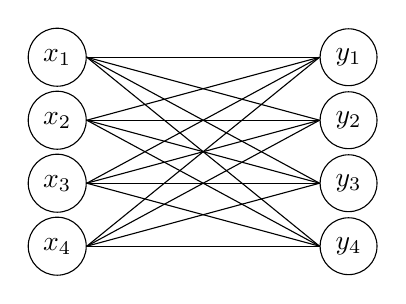
\begin{tikzpicture}
  \foreach \i/\y in {1/3.8, 2/3.0, 3/2.2, 4/1.4} {
    \node[draw, rounded corners=0.1pt, shape=circle] (x\i) at (0,\y) {$x_\i$};
    \node[draw, rounded corners=0.1pt, shape=circle] (y\i) at (3.7,\y) {$y_\i$};
  }

  \foreach \i in {1,...,4} {
    \foreach \j in {1,...,4} {
      \draw (x\j.east) -- (y\i.west);
    }
  }
\end{tikzpicture}
}
  }
  \only<2>{\resizebox{0.8\textwidth}{!}{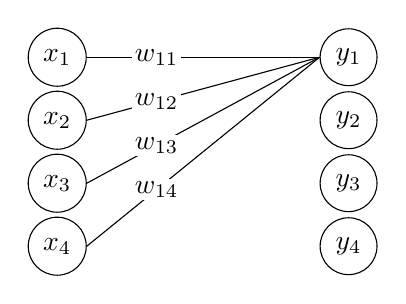
\begin{tikzpicture}
  \foreach \i/\y in {1/3.8, 2/3.0, 3/2.2, 4/1.4} {
    \node[draw, rounded corners=0.1pt, shape=circle] (x\i) at (0,\y) {$x_\i$};
    \node[draw, rounded corners=0.1pt, shape=circle] (y\i) at (3.7,\y) {$y_\i$};
  }

  \foreach \j in {1,...,4} {
    \draw (x\j.east) -- node[pos=0.3, fill=white, inner sep=1pt] {$w_{1\j}$} (y1.west);
  }
\end{tikzpicture}
}
    \[y_1 = x_1 w_{11} + x_2 w_{12} + x_3 w_{13} + x_4 w_{14}\]
  }
  \only<3>{\resizebox{0.8\textwidth}{!}{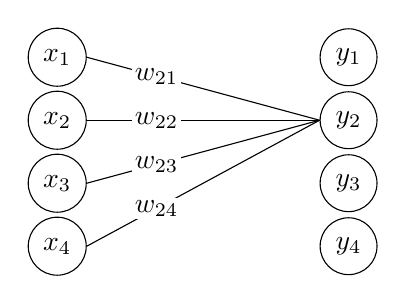
\begin{tikzpicture}
  \foreach \i/\y in {1/3.8, 2/3.0, 3/2.2, 4/1.4} {
    \node[draw, rounded corners=0.1pt, shape=circle] (x\i) at (0,\y) {$x_\i$};
    \node[draw, rounded corners=0.1pt, shape=circle] (y\i) at (3.7,\y) {$y_\i$};
  }

  \foreach \j in {1,...,4} {
    \draw (x\j.east) -- node[pos=0.3, fill=white, inner sep=1pt] {$w_{2\j}$} (y2.west);
  }
\end{tikzpicture}
}
    \[y_2 = x_1 w_{21} + x_2 w_{22} + x_3 w_{23} + x_4 w_{24}\]
  }
  \only<4>{\resizebox{0.8\textwidth}{!}{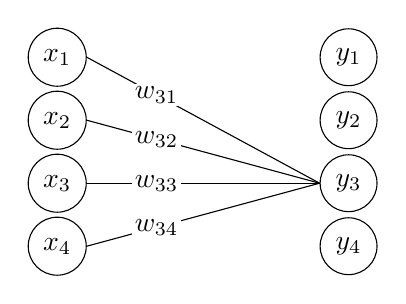
\begin{tikzpicture}
  \foreach \i/\y in {1/3.8, 2/3.0, 3/2.2, 4/1.4} {
    \node[draw, rounded corners=0.1pt, shape=circle] (x\i) at (0,\y) {$x_\i$};
    \node[draw, rounded corners=0.1pt, shape=circle] (y\i) at (3.7,\y) {$y_\i$};
  }

  \foreach \j in {1,...,4} {
    \draw (x\j.east) -- node[pos=0.3, fill=white, inner sep=1pt] {$w_{3\j}$} (y3.west);
  }
\end{tikzpicture}
}
    \[y_3 = x_1 w_{31} + x_2 w_{32} + x_3 w_{33} + x_4 w_{34}\]
  }
  \only<5>{\resizebox{0.8\textwidth}{!}{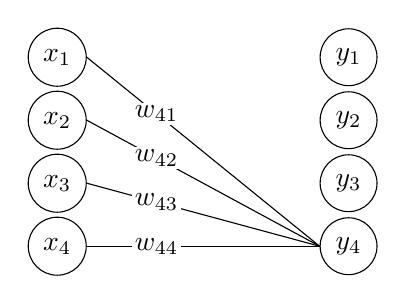
\begin{tikzpicture}
  \foreach \i/\y in {1/3.8, 2/3.0, 3/2.2, 4/1.4} {
    \node[draw, rounded corners=0.1pt, shape=circle] (x\i) at (0,\y) {$x_\i$};
    \node[draw, rounded corners=0.1pt, shape=circle] (y\i) at (3.7,\y) {$y_\i$};
  }

  \foreach \j in {1,...,4} {
    \draw (x\j.east) -- node[pos=0.3, fill=white, inner sep=1pt] {$w_{4\j}$} (y4.west);
  }
\end{tikzpicture}
}
    \[y_4 = x_1 w_{41} + x_2 w_{42} + x_3 w_{43} + x_4 w_{44}\]
  }
\end{frame}

\begin{frame}
  \frametitle{Linear Algebra Interpretation}
  Here, notice that for each \(y_i\), we are taking a weighted sum of the
  \(x\) elements. That is,

  \[y_i = x_1 w_{i1} + x_2 w_{i2} + x_3 w_{i3} + x_4w_{i4}.\]

  Arranging the \(y_i\) into a vector, we get

  \[
    \begin{bmatrix}
      y_1 \\ y_2 \\ y_3 \\ y_4
    \end{bmatrix}
    =
    \begin{bmatrix}
      w_{11} & w_{12} & w_{13} & w_{14} \\
      w_{21} & w_{22} & w_{23} & w_{24} \\
      w_{31} & w_{32} & w_{33} & w_{34} \\
      w_{41} & w_{42} & w_{43} & w_{44}
    \end{bmatrix}
    \begin{bmatrix}
      x_1 \\ x_2 \\ x_3 \\ x_4
    \end{bmatrix}.
  \]

\end{frame}

\begin{frame}
  \frametitle{Linear Algebra Interpretation}
  We can generalize the number of \(x\)'s and the number of \(y\)'s.

  \[
    \begin{bmatrix}
      y_1 \\ y_2 \\ \vdots \\ y_m
    \end{bmatrix}
    =
    \begin{bmatrix}
      w_{11} & w_{12} & \cdots & w_{1n} \\
      w_{21} & w_{22} & \cdots & w_{2n} \\
      \vdots & \vdots & \ddots & \vdots \\
      w_{m1} & w_{m2} & \cdots & w_{mn}
    \end{bmatrix}
    \begin{bmatrix}
      x_1 \\ x_2 \\ \vdots \\ x_n
    \end{bmatrix}.
  \]

  We say, \(n\) is the \emph{input dimension} and \(m\) is the \emph{output dimension}.
\end{frame}
\begin{frame}
  \frametitle{Computing with multiple \(x\) vectors.}
  Suppose we have multiple \(x\) vectors, for which we want to pass through our
  neural network. We can stack the multiple \(x\) vectors in the \textbf{batch},
  which we compute with a matrix multiplication.

  \[
    \resizebox{\textwidth}{!}{$\displaystyle
      \begin{bmatrix}
        y_1^{(1)} & y_1^{(2)} & \cdots & y_1^{(B)} \\
        y_2^{(1)} & y_2^{(2)} & \cdots & y_2^{(B)} \\
        \vdots & \vdots & \ddots & \vdots \\
        y_m^{(1)} & y_m^{(2)} & \cdots & y_m^{(B)}
      \end{bmatrix}
      =
      \begin{bmatrix}
        w_{11} & w_{12} & \cdots & w_{1n} \\
        w_{21} & w_{22} & \cdots & w_{2n} \\
        \vdots & \vdots & \ddots & \vdots \\
        w_{m1} & w_{m2} & \cdots & w_{mn}
      \end{bmatrix}
      \begin{bmatrix}
        x_1^{(1)} & x_1^{(2)} & \cdots & x_1^{(B)} \\
        x_2^{(1)} & x_2^{(2)} & \cdots & x_2^{(B)} \\
        \vdots & \vdots & \ddots & \vdots \\
        x_n^{(1)} & x_n^{(2)} & \cdots & x_n^{(B)}
      \end{bmatrix}.
    $}
  \]

  We write this succinctly as \(Y = WX\), where \(Y \in \mathbb{R}^{m \times B}\),
  \(X \in \mathbb{R}^{n \times B}\), and \(W \in \mathbb{R}^{m \times n}\).

  \begin{alertblock}{New Representation}
    We have successfully mapped the batched computation of a \textbf{linear layer}
    a matrix multiplication!
  \end{alertblock}
\end{frame}

\begin{frame}
  \frametitle{Composing Layers}

  We can view \(W\) as a function that takes in an \(n\)-dimensional vector and
  maps it to an \(m\)-dimensional vector. \(W \colon \mathbb{R}^n \rightarrow \mathbb{R}^m\).
  We create deep neural networks by \emph{composing} these transformations, along
  with  \textbf{nonlinearities} \(\sigma_i\).

  \begin{center}
  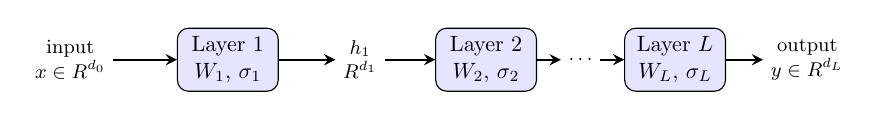
\begin{tikzpicture}[
    scale=0.8, transform shape,
    >=stealth,
    layer/.style={draw, rounded corners, fill=blue!10,
      minimum width=1.6cm, minimum height=1cm, align=center},
    value/.style={align=center, font=\small}
  ]
    \node[value] (x) at (0,0) {input\\\(x \in \mathbb{R}^{d_0}\)};
    \node[layer] (l1) at (2.5,0) {Layer 1\\\(W_1,\,\sigma_1\)};
    \node[value] (h1) at (4.6,0) {\(h_1\)\\\(\mathbb{R}^{d_1}\)};
    \node[layer] (l2) at (6.6,0) {Layer 2\\\(W_2,\,\sigma_2\)};
    \node[value] (dots) at (8.1,0) {\(\cdots\)};
    \node[layer] (lL) at (9.6,0) {Layer \(L\)\\\(W_L,\,\sigma_L\)};
    \node[value] (y) at (11.7,0) {output\\\(y \in \mathbb{R}^{d_L}\)};

    \draw[->, thick] (x) -- (l1);
    \draw[->, thick] (l1) -- (h1);
    \draw[->, thick] (h1) -- (l2);
    \draw[->, thick] (l2) -- (dots);
    \draw[->, thick] (dots) -- (lL);
    \draw[->, thick] (lL) -- (y);
  \end{tikzpicture}

  \medskip
  \(h_0=x,\qquad h_\ell=\sigma_\ell(W_\ell h_{\ell-1}),\qquad y=h_L\)
\end{center}


  \begin{block}{Remark}
    Notice that this figure doesn't show the \emph{batch} dimension. However,
    if you work through the dimension mappings, the \emph{batch} dimension \(B\)
    will be unaffected by this composition.
  \end{block}
\end{frame}

\begin{frame}
  \frametitle{Limitations for Neural Network Architecture}

  \begin{center}
  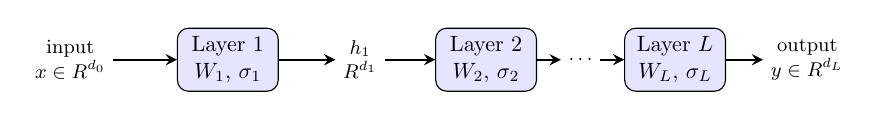
\begin{tikzpicture}[
    scale=0.8, transform shape,
    >=stealth,
    layer/.style={draw, rounded corners, fill=blue!10,
      minimum width=1.6cm, minimum height=1cm, align=center},
    value/.style={align=center, font=\small}
  ]
    \node[value] (x) at (0,0) {input\\\(x \in \mathbb{R}^{d_0}\)};
    \node[layer] (l1) at (2.5,0) {Layer 1\\\(W_1,\,\sigma_1\)};
    \node[value] (h1) at (4.6,0) {\(h_1\)\\\(\mathbb{R}^{d_1}\)};
    \node[layer] (l2) at (6.6,0) {Layer 2\\\(W_2,\,\sigma_2\)};
    \node[value] (dots) at (8.1,0) {\(\cdots\)};
    \node[layer] (lL) at (9.6,0) {Layer \(L\)\\\(W_L,\,\sigma_L\)};
    \node[value] (y) at (11.7,0) {output\\\(y \in \mathbb{R}^{d_L}\)};

    \draw[->, thick] (x) -- (l1);
    \draw[->, thick] (l1) -- (h1);
    \draw[->, thick] (h1) -- (l2);
    \draw[->, thick] (l2) -- (dots);
    \draw[->, thick] (dots) -- (lL);
    \draw[->, thick] (lL) -- (y);
  \end{tikzpicture}

  \medskip
  \(h_0=x,\qquad h_\ell=\sigma_\ell(W_\ell h_{\ell-1}),\qquad y=h_L\)
\end{center}


  Architectures such as \textbf{Transformers} and \textbf{CNNs} have connectivity
  patterns more complex than a simple composition of layers. Nevertheless, linear
  transformations remain a fundamental computational primitive in neural network
  architectures.

  \begin{block}{A fundamental building block}
    A linear transformation may seem like a narrow operation to study, but modern
    neural networks perform it repeatedly and at enormous scale. Its efficiency
    therefore has an outsized effect on training and inference performance. The
    rest of this presentation explores the hardware and techniques that make these
    operations efficient.
  \end{block}

\end{frame}

\begin{frame}
  \frametitle{Takeaways}
  \begin{enumerate}
    \item A linear layer applied to a batch of inputs can be expressed as a single
      matrix multiplication, \(Y = WX\).
    \item Deep networks compose these linear transformations with nonlinearities.
      More complex architectures change how layers are connected, but linear
      transformations remain a fundamental building block.
    \item \textbf{Matrix multiplication therefore captures a large and reusable part of
      neural network computation.}
  \end{enumerate}

  \begin{alertblock}{Why is this representation useful?}
    It separates what the network computes from how the hardware executes it.
    Instead of optimizing every architecture from scratch, we can focus on one
    common computational primitive. Next, we will examine how GPUs execute matrix
    multiplications efficiently.
  \end{alertblock}
\end{frame}

\end{document}
